\documentclass{beamer}\usepackage{graphicx, color}
%% maxwidth is the original width if it is less than linewidth
%% otherwise use linewidth (to make sure the graphics do not exceed the margin)
\makeatletter
\def\maxwidth{ %
  \ifdim\Gin@nat@width>\linewidth
    \linewidth
  \else
    \Gin@nat@width
  \fi
}
\makeatother

\IfFileExists{upquote.sty}{\usepackage{upquote}}{}
\definecolor{fgcolor}{rgb}{0.2, 0.2, 0.2}
\newcommand{\hlnumber}[1]{\textcolor[rgb]{0,0,0}{#1}}%
\newcommand{\hlfunctioncall}[1]{\textcolor[rgb]{0.501960784313725,0,0.329411764705882}{\textbf{#1}}}%
\newcommand{\hlstring}[1]{\textcolor[rgb]{0.6,0.6,1}{#1}}%
\newcommand{\hlkeyword}[1]{\textcolor[rgb]{0,0,0}{\textbf{#1}}}%
\newcommand{\hlargument}[1]{\textcolor[rgb]{0.690196078431373,0.250980392156863,0.0196078431372549}{#1}}%
\newcommand{\hlcomment}[1]{\textcolor[rgb]{0.180392156862745,0.6,0.341176470588235}{#1}}%
\newcommand{\hlroxygencomment}[1]{\textcolor[rgb]{0.43921568627451,0.47843137254902,0.701960784313725}{#1}}%
\newcommand{\hlformalargs}[1]{\textcolor[rgb]{0.690196078431373,0.250980392156863,0.0196078431372549}{#1}}%
\newcommand{\hleqformalargs}[1]{\textcolor[rgb]{0.690196078431373,0.250980392156863,0.0196078431372549}{#1}}%
\newcommand{\hlassignement}[1]{\textcolor[rgb]{0,0,0}{\textbf{#1}}}%
\newcommand{\hlpackage}[1]{\textcolor[rgb]{0.588235294117647,0.709803921568627,0.145098039215686}{#1}}%
\newcommand{\hlslot}[1]{\textit{#1}}%
\newcommand{\hlsymbol}[1]{\textcolor[rgb]{0,0,0}{#1}}%
\newcommand{\hlprompt}[1]{\textcolor[rgb]{0.2,0.2,0.2}{#1}}%

\usepackage{framed}
\makeatletter
\newenvironment{kframe}{%
 \def\at@end@of@kframe{}%
 \ifinner\ifhmode%
  \def\at@end@of@kframe{\end{minipage}}%
  \begin{minipage}{\columnwidth}%
 \fi\fi%
 \def\FrameCommand##1{\hskip\@totalleftmargin \hskip-\fboxsep
 \colorbox{shadecolor}{##1}\hskip-\fboxsep
     % There is no \\@totalrightmargin, so:
     \hskip-\linewidth \hskip-\@totalleftmargin \hskip\columnwidth}%
 \MakeFramed {\advance\hsize-\width
   \@totalleftmargin\z@ \linewidth\hsize
   \@setminipage}}%
 {\par\unskip\endMakeFramed%
 \at@end@of@kframe}
\makeatother

\definecolor{shadecolor}{rgb}{.97, .97, .97}
\definecolor{messagecolor}{rgb}{0, 0, 0}
\definecolor{warningcolor}{rgb}{1, 0, 1}
\definecolor{errorcolor}{rgb}{1, 0, 0}
\newenvironment{knitrout}{}{} % an empty environment to be redefined in TeX

\usepackage{alltt}
\usetheme{Stats}
\setbeamercovered{transparent}
\usepackage{color}
\usepackage{hyperref}
  \hypersetup{
  	colorlinks=true
		linkcolor=black
		}
\usepackage{url}
\usepackage{graphics}
\usepackage{tikz}
\usepackage{booktabs}





%%%%%%%%%%%%%%%%%%%%%%%%%%%%%%%% Title Slide %%%%%%%%%%%%%%%%%%%%%%%%%%
\title[]{Intro to Social Science Data Analysis \\[1cm] Lecture 10: Comparing Proportions \& Simple Linear Regression}
\author[]{
    \href{mailto:gandrud@yonsei.ac.kr}{Christopher Gandrud}
}
\date{\today}


\begin{document}

\frame{\titlepage}

\section[Outline]{}
\frame{\tableofcontents}

%%%%%%%%%%%% Assignment 3
\section{Assignment 3}
\frame{
  \frametitle{Assignment 3}
  {\Large{Assignment 3}} \\[0.5cm]
  {\bf{Due:}} Friday 16 November \\[0.5cm]
  Have a data set with three variables of the following type:
  \begin{itemize}
    \item 1 numeric variable,
    \item 1 dummy variable,
    \item 1 multinomial variable.
  \end{itemize}
  There should be more than 50 observations per variable \& variable category.
}

\frame{
  \frametitle{Assignment 3}
  {\Large{Find the answers to these questions.}} \\[0.5cm]
Numeric Continuous Variable
  \begin{itemize}
    \item What do you predict the population mean of this variable is? 
    \item Create two groups of this variable based on the dummy variable. Are the population means of these two groups likely to be different? (extra points if you can show this graphically)
  \end{itemize}
Categorical Variables
  \begin{itemize}
    \item Do the two groups of the dummy variable have values on the multinomial variable that are independent of one another? 
  \end{itemize}
}

%%%%%%%%%%%%% Recap
\section{Recap}
\frame{
	\frametitle{Quick Quiz (1)}
  Create a hypothesis test to examine whether infant morality rates are on average different in OECD countries compared to non-OECD countries.
}

\frame{
  \frametitle{Quick Quiz (2)}
  What conditions do we need to meet in order to use the Central Limit Theorem to assume that our sampling distribution is normally distributed? \\[0.5cm]
  If we have a small sample size ($< 50$) what alternative sampling distribution could we use?
}

\frame{
  \frametitle{Quick Quiz (3)}
  What is a p-value? \\[0.5cm]
  What two steps do you take to calculate a p-value? \\[0.5cm]
  How does a p-value compare to a confidence interval?
}


%%%%%%%%%%%%% X^2 test statistic
\section{Inferring the Distribution of Population Proportions: the $\chi^2$ test statistic}
\frame{
  \frametitle{Today, Part I}
{\Large{Last class we learned how to draw inferences from sample means.}} \\[0.5cm]
{\Large{This is useful for continuous numeric variables, but what if we have {\bf{categorical variables}}?}}
}

\frame{
  \frametitle{Today, Part I}
{\Large{In the first part of today's lecture we will learn how to make inferences from {\bf{sample proportions}}.}}
}

\frame{
  \frametitle{Mode}
{\LARGE{Remember the Mode:}} \\[0.5cm]
  For categorical variables the best measure of central tendency is the {\bf{mode}}. \\[0.5cm]
  A way of measuring the mode in a {\bf{meaningfully comparable way}} is with {\bf{proportions}}. \\[0.5cm]
  In general, for categorical data we are interested in {\bf{inferring population proportions}}. These proportions are our {\bf{population parameter}} of interest.
}

\frame{
  \frametitle{Quick Quiz}
  Imagine we have a random sample of 275 juries in a US country. Overall the juries have the following racial composition:
  \begin{table}
    \begin{tabular}{c c c c c}
    \hline
    White & Black & Hispanic & Other & Total \\
    \hline\hline
    205 & 26 & 25 & 19 & 275 \\ 
    \hline
    \end{tabular}
  \end{table}
  With a partner find the {\bf{sample proportions}} for each racial group. \\[0.5cm]
  Example from Diaz et al. Ch. 5.
}

\begin{frame}[fragile]
  \frametitle{Sampling Proportions}
  \begin{table}
    \caption{Racial Composition of Sample Juries}
    \begin{tabular}{l c c c c c}
    \hline
    & White & Black & Hispanic & Other & Total \\
    \hline\hline
    Sample Count & 205 & 26 & 25 & 19 & 275 \\ 
    Sample Proportion & 0.75 & 0.09 & 0.09 & 0.07 & 1 \\
    \hline
    \end{tabular}
  \end{table}
\end{frame}

\frame{
  \frametitle{Question}
{\Large{Is the racial composition of the juries similar to the racial composition of the county's population?}}
}

\begin{frame}[fragile]
  \frametitle{Sampling Proportions vs. Population Proportions}
  \begin{table}
    \caption{Racial Composition of Sample Juries \& County's Registered Voters}
    \begin{tabular}{l c c c c c}
    \hline
    & White & Black & Hispanic & Other & Total \\
    \hline\hline
    Sample Count & 205 & 26 & 25 & 19 & 275 \\ 
    Sample Proportion & 0.75 & 0.09 & 0.09 & 0.07 & 1 \\ \hline
    Registered Voters & 0.72 & 0.07 & 0.12 & 0.09 & 1 \\
    \hline
    \end{tabular}
  \end{table}
\end{frame}

\frame{
  \frametitle{Sample vs. Population}
{\Large{They are different, but are they {\bf{statistically different}} or is the difference simply due to {\bf{sampling error}}?}}
}

\frame{
  \frametitle{Hypothesis Testing}
{\LARGE{Null Hypothesis:}} \\[0.5cm]
  $H_{0}:$ The jurors are randomly sampled from the county's population. There is no racial bias in jury selection. \\[0.5cm]
  
{\LARGE{Alternative Hypothesis:}} \\[0.5cm]
  $H_{A}:$ The jurors are not randomly sampled, i.e. there is racial bias in juror selection.
}

\frame{
\begin{center}
{\LARGE{How do we test these hypotheses?}}
\end{center}
}

\begin{frame}[fragile]
  \frametitle{1st the Test Statistic}
  Last week we used the following equation for a {\bf{test statistic}}:
  \[
  \frac{\mathrm{point\:estimate} - \mathrm{null\:value}}{\mathrm{SE\:of\:the\:point\:estimate}}
  \] \\[0.5cm]
  Let's use a similar strategy to find the test statistic for the proportions.
\end{frame}

\frame{
\begin{center}
{\LARGE{What is the null value?}}
\end{center}
}

\begin{frame}[fragile]
  \frametitle{Null Value for Proportions}
  Our null value is the {\bf{expected frequencies in the sample}} if the {\bf{null hypothesis is true}}.
  \begin{table}
    \caption{Expected Racial Composition if Null Hypothesis is True}
    \begin{tabular}{l c c c c c}
    \hline
    & White & Black & Hispanic & Other & Total \\
    \hline\hline
    Sample Count & 205 & 26 & 25 & 19 & 275 \\ 
    Registered Voters & 0.72 & 0.07 & 0.12 & 0.09 & 1 \\ \hline
    Expected Frequency & 198 & 19.25 & 33 & 24.75 & 275 \\
    \hline
    \end{tabular}
  \end{table}
\end{frame}

\begin{frame}[fragile]
 \frametitle{The Test Statistic (1)}
 Now we can calculate the test statistic for {\emph{white}} jurors. \\[0.5cm]
 \[
 Z_{white} = \frac{205 - 198}{\sqrt{198}} = 0.5
 \]
 
 {\bf{Note:}} in this case the standard error is the square root of the expected count under the null hypothesis.
\end{frame}

\begin{frame}[fragile]
 \frametitle{The Test Statistic (2)}
 We can also calculate the test statistic for the other racial groups. \\[0.5cm]
 \[
 Z_{black} = \frac{26 - 19.25}{\sqrt{19.25}} = 1.54
 \] \\[0.3cm]
  \[
 Z_{hispanic} = \frac{25 - 33}{\sqrt{33}} = -1.39
 \]\\[0.3cm]
  \[
 Z_{other} = \frac{19 - 24.75}{\sqrt{24.25}} = -1.16
 \]\\[0.3cm]
\end{frame}

\frame{
  \frametitle{$\chi^{2}$ (1)}
  Our hypotheses were about whether {\bf{all}} of the sample proportions were different from the population proportions. \\[0.5cm]
  How can we combine these four test statistics together?
}

\frame{
  \frametitle{$\chi^{2}$ (1)}
{\LARGE{$\chi^{2}$ test statistic:}} \\[0.5cm]
  \[
  \chi^{2} = Z^{2}_{1} + Z^{2}_{2} \ldots Z^{2}_{n}
  \] \\[0.5cm]
  For our example this would be:
  \[
  \chi^{2} = 0.5^{2} + 1.54^{2} + -1.39^{2} + -1.16^{2} = 5.89
  \] \\[0.5cm]
  Note: {$\chi^{2}$} is pronounced ``ki squared".
}

\frame{
  \frametitle{$\chi^{2}$ Distribution}
  We {\bf{can't}} assume that the $\chi^{2}$ statistic follows a normal or $t$ distribution if the null hypothesis is true. \\[0.5cm]
  Instead, we use a {\bf{$\chi^{2}$ distribution}}. \\[0.5cm]
  It's only parameter is {\bf{degrees of freedom}} ($df$). \\[0.25cm]
  If $k$ is the {\bf{number of categories}} then  
  \[
  df = k - 1
  \] 
}

\frame{
  \frametitle{The $\chi^{2}$ distribution with various degrees of freedom}
  \begin{center}
    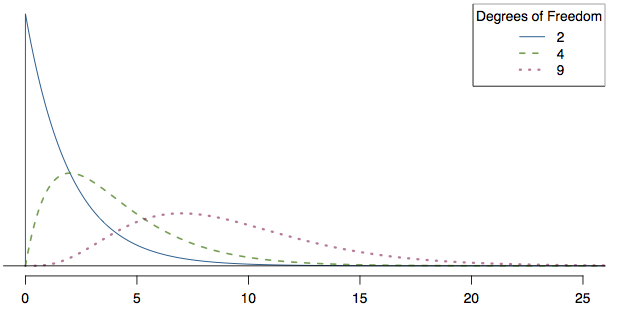
\includegraphics[scale=0.5]{Chi2.png}
    \\[0.25cm]
  \end{center}
{\tiny{Diaz et al. (2011, 216)}}
}

\frame{
  \frametitle{Our Example}
  In our example we have:
  \[
  \chi^{2} = 5.89
  \]
  \[
  df = 4 - 1 = 3
  \] \\[0.5cm]
  What is the probability of finding data at least as favourable to the alternative hypothesis as this, if the null hypothesis was true?
}

\frame{
  \frametitle{The $\chi^{2}$ distribution with 3 degrees of freedom}
  \begin{center}
    \includegraphics[scale=0.6]{Chi2specific.png}
    \\[0.25cm]
  \end{center}
{\tiny{Diaz et al. (2011, 219)}}
}

\begin{frame}[fragile]
  \frametitle{Finding the p-value in R}
  To find the p-value in R for $\chi^{2}$ of 5.89 when there are 3 degrees of freedom:
\begin{knitrout}
\definecolor{shadecolor}{rgb}{0.969, 0.969, 0.969}\color{fgcolor}\begin{kframe}
\begin{alltt}
\hlcomment{# Find p-value}
1 - \hlfunctioncall{pchisq}(q = 5.89, df = 3)
\end{alltt}
\begin{verbatim}
## [1] 0.1171
\end{verbatim}
\end{kframe}
\end{knitrout}


At the 95\% significance level we fail to reject the null hypothesis that the jurors are randomly chosen from the country population.
\end{frame}

\frame{
  \frametitle{Conditions for the $\chi^{2}$ Test}
{\LARGE{Conditions for the $\chi^{2}$ Test:}} \\[0.5cm]
  \begin{itemize}
    \item Each case that contributes a count must be {\bf{independent}} of the other cases.
    \item Each cell count must be {\bf{10 or greater}}.
  \end{itemize}
}

%%%%%%%%%%% X^2 for comparing group proportions
\section{$\chi^{2}$ Test of Independence}
\frame{
  \frametitle{Test of Group Independence}
{\Large{We can use a similar test to examine if groups in samples are different, i.e. if they are {\bf{independent}}}}
}

\frame{
  \frametitle{Question}
  \begin{center}
{\LARGE{Do disadvantaged children who attended preschool have better life outcomes than children who did not go to preschool?}}
  \end{center}
}

\frame{
  \frametitle{Abecedarian Study Data (Campbell et al., 2002)}
  \begin{table}
    \caption{Two-way Contingency Table of Selected Data Age 21 Follow-Up Data from the Abecefarian Study}
    \begin{tabular}{p{2.cm} c c c | c}
    \hline
    & & Preschool & No Preschool  & Total \\
    \hline\hline
    University Enrolment & Enrolled & 37 & 7 & 44\\
    &Not Enrolled & 16 & 44 & 60 \\
    \hline
    Total & & 53 & 51 & 104 \\
    \hline
    \end{tabular}
  \end{table}
}

\frame{
  \frametitle{Hypothesis Testing}
{\LARGE{Null Hypothesis:}} \\[0.5cm]
  $H_{0}:$ There is no difference in university enrolment at age 21 between disadvantaged children who attended preschool and those who didn't. (dependent) \\[0.5cm]
  
{\LARGE{Alternative Hypothesis:}} \\[0.5cm]
  $H_{A}:$ There is a difference in university enrolment at age 21 between disadvantaged children who attended preschool and those who didn't. (independent)
}

\frame{
  \frametitle{Test Statistic (1)}
  First find the expected counts if the null hypothesis was true. \\[0.5cm]
  We observe that 44 of the 104 people attend university. This is a proportion of:
  \[
  \frac{44}{104} = 0.423
  \] \\[0.5cm]
  So we would expect that the number of people who attended preschool and are now in university would be:
  \[
  0.423 * 53 = 22.42
  \]
}

\frame{
  \frametitle{General Frequency Count Equation}
  The general formula for finding the {\bf{expected count}} for a row $i$ in column $j$ is:
  \[
  \mathrm{Expected\:Count_{i, j}} = \frac{(\mathrm{row}\:i\:\mathrm{total}) * (\mathrm{column}\:j\:\mathrm{total})}{n}
  \]
}

\frame{
  \frametitle{Expected vs. Observed Counts in Two-way Contingency Tables}
{\scriptsize{
  \begin{table}
    \caption{Expected vs. Observed Counts}
    \begin{tabular}{p{2cm} c c c c c | c}
    \hline
    & & Pres. & & No Pres. & & Total \\
    \hline\hline
    University Enrolment & Enrolled & 37 & (22.42) & 7 & (21.57) & 44\\
    &Not Enrolled & 16 & (30.58) & 44 & (29.43) & 60 \\
    \hline
    Total & & 53 & & 51 & & 104 \\
    \hline
    \end{tabular}
  \end{table}
}}
  Note: Expected counts in parentheses.
}

\frame{
  \frametitle{Test Statistic (2)}
  Now we find the test statistic in a similar way to what we did with the one-way table. \\[0.5cm]
  If $f_{o}$ is the observed frequency and $f_{e}$ is the expected frequency, then:
  \[
  \chi^{2} = \sum\left[\frac{(f_{o} - f_{e})^2}{f_{e}}\right]
  \]\\[0.5cm]
  The equation for the degrees of freedom ($df$) is a little different:
  \[
  df = (\mathrm{number\:of\:rows} - 1) * (\mathrm{number\:of\:columns} - 1)
  \]
}

\frame{
  \frametitle{Finding $\chi^{2}$ \& $df$}
  \[
    \chi^{2} = 9.48 + 9.842 + 6.951 + 7.213 = 33.486
  \]\\[0.5cm]
  \[
  df = (2 - 1) * (2 - 1) = 1
  \]
}

\begin{frame}[fragile]
  \frametitle{Finding the p-value in R}
  To find the p-value in R for $\chi^{2}$ of 33.486 when there is 1 degree of freedom:
\begin{knitrout}
\definecolor{shadecolor}{rgb}{0.969, 0.969, 0.969}\color{fgcolor}\begin{kframe}
\begin{alltt}
\hlcomment{# Find p-value}
1 - \hlfunctioncall{pchisq}(q = 33.486, df = 1)
\end{alltt}
\begin{verbatim}
## [1] 7.178e-09
\end{verbatim}
\end{kframe}
\end{knitrout}


At the 95\% significance level we reject the null hypothesis that there is no difference in university enrolment at age 21 between the people who attended preschool and those who didn't.
\end{frame}

\begin{frame}[fragile]
  To do this in R (the easy way):
\begin{knitrout}
\definecolor{shadecolor}{rgb}{0.969, 0.969, 0.969}\color{fgcolor}\begin{kframe}
\begin{alltt}
\hlcomment{# Create Contingency Table}
Preschool <- \hlfunctioncall{c}(37, 16)
NoPreschool <- \hlfunctioncall{c}(7, 44)
Data <- \hlfunctioncall{data.frame}(Preschool, NoPreschool)

\hlcomment{# Find chi2 and p-value}
\hlfunctioncall{chisq.test}(Data)
\end{alltt}
\begin{verbatim}
## 
## 	Pearson's Chi-squared test with Yates'
## 	continuity correction
## 
## data:  Data 
## X-squared = 31.24, df = 1, p-value =
## 2.284e-08
\end{verbatim}
\end{kframe}
\end{knitrout}

\end{frame}

\frame{
  See also: \url{http://www.r-tutor.com/elementary-statistics/goodness-fit/chi-squared-test-independence}.
}

%%%%%%%%% Introduction to Simple Linear Regression
\section{Introduction to Simple Linear Regression}
\frame{
  \frametitle{Inference so far\ldots}
  So far we have used tools of statistical inference to determine
  \begin{itemize}
    \item<1-> likely population parameters from a sample, especially the mean \& proportions, 
    \item<1-> if groups are independent.
  \end{itemize}\\[0.5cm]
  What if we want to use the value of one variable to predict the value of another variable?\\ Or at least describe the relationship between variables in more detail than ``they are independent or not"?
}

\frame{
  \frametitle{Introduction to Simple Linear Regression}
  \begin{center}
{\LARGE{Simple Linear Regression}}
  \end{center}
}

\frame{
  \frametitle{Question}
  \begin{center}
  How closely does a high school GPA predict someone's university GPA?
  \end{center}
}

\begin{frame}[fragile]
  If there was a perfect linear relationship we would expect to see data like this:\\[0.5cm]
\begin{knitrout}
\definecolor{shadecolor}{rgb}{0.969, 0.969, 0.969}\color{fgcolor}

{\centering 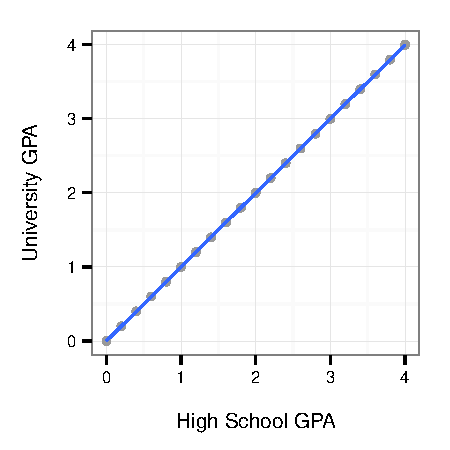
\includegraphics[width=\maxwidth]{figure/PerfectLinear} 

}


\end{knitrout}

\end{frame}

\frame{
  \frametitle{Simplest Equation}
  We could describe this relationship with the following equation: \\[0.5cm]
  If University GPA is denoted $y$ and High School GPA is denoted $x$
  \[
  y = x
  \]
}

\frame{
  \frametitle{More General Equation}
  We could use a slightly more general equation: \\[0.5cm]
  If $\alpha$ is the line's {\bf{y-intercept}} and $\beta$ ({\bf{coefficient}}) is the slope of the line then:
  \[
  y = \alpha + \beta x
  \] \\[0.5cm]
  This is known as the {\bf{simple linear regression equation}}. 
}

\begin{frame}[fragile]
  \\[0.5cm]
\begin{knitrout}
\definecolor{shadecolor}{rgb}{0.969, 0.969, 0.969}\color{fgcolor}

{\centering 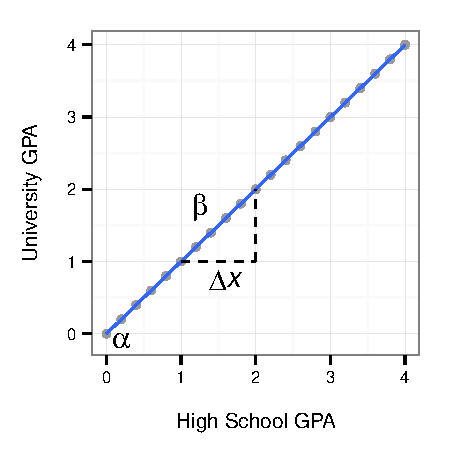
\includegraphics[width=\maxwidth]{figure/PerfectLinearExplain} 

}


\end{knitrout}

\end{frame}


\frame{
  \frametitle{Perfectly Predicts}
  In our example if High School GPA perfectly predicts University GPA than we would have the full equation:
  \[
  y = \alpha + \beta x = 0 + 1 * x = x
  \]
}

\frame{
  \frametitle{Interpreting $\beta$}
{\LARGE{Interpreting $\beta$:}} \\[0.5cm]
  For every one unit increase in $x$  ($ + \Delta x $) we expect $\beta$ unit increase in $y$. \\[0.5cm]
  In our example, for every 1 point increase in High School GPA we expect a 1 unit increase in University GPA.
}

\frame{
  \frametitle{Question}
  What would the simple linear regression equation be if everybody's University GPA was exactly 1 point higher than their High School GPA?
}

\frame{
  \frametitle{}
  \[
  y = 1 + \beta x
  \]
}



\begin{frame}[fragile]
  \\[0.5cm]
\begin{knitrout}
\definecolor{shadecolor}{rgb}{0.969, 0.969, 0.969}\color{fgcolor}

{\centering 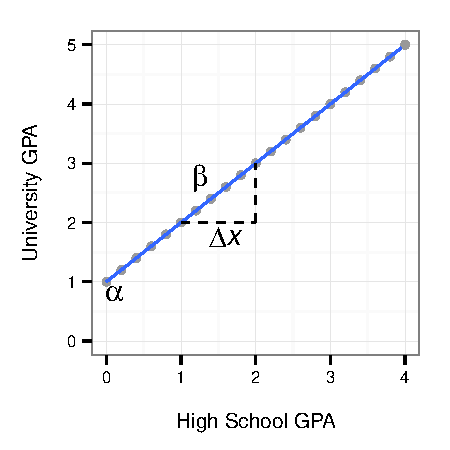
\includegraphics[width=\maxwidth]{figure/PerfectLinearExplain2} 

}


\end{knitrout}

\end{frame}

\frame{
  \frametitle{Question}
  What would the simple linear regression equation be if University GPA was half High School GPA?
}

\frame{
  \frametitle{}
  \[
  y = 0 + 0.5(x)
  \]
}

\begin{frame}[fragile]
  \\[0.5cm]
\begin{knitrout}
\definecolor{shadecolor}{rgb}{0.969, 0.969, 0.969}\color{fgcolor}

{\centering 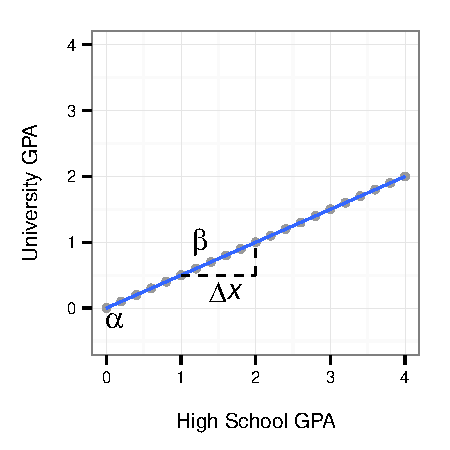
\includegraphics[width=\maxwidth]{figure/PerfectLinearExplain4} 

}


\end{knitrout}

\end{frame}

\frame{
  \frametitle{Question}
  What would the simple linear regression equation be if University GPA was one times less than High School GPA?
}

\frame{
  \frametitle{}
  \[
  y = 0 - 1(x)
  \]
}

\begin{frame}[fragile]
  \\[0.5cm]
\begin{knitrout}
\definecolor{shadecolor}{rgb}{0.969, 0.969, 0.969}\color{fgcolor}

{\centering 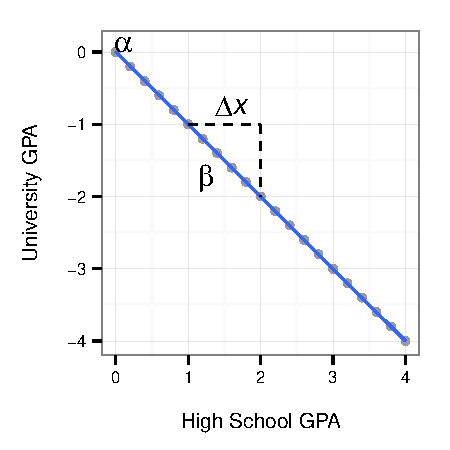
\includegraphics[width=\maxwidth]{figure/PerfectLinearExplain5} 

}


\end{knitrout}

\end{frame}

\frame{
  \frametitle{Direction of the Relationship}
{\LARGE{Negative Relationship:}} \\[0.5cm]
  A relationship between variables $x$ and $y$ is negative if the regression coefficient is negative. \\[0.5cm]
{\LARGE{Positive Relationship:}} \\[0.5cm]
  A relationship between variables $x$ and $y$ is positive if the regression coefficient is negative.
}

\frame{
  \frametitle{But\ldots}
  \begin{center}
{\LARGE{Of course, real world relationships are {\bf{rarely}} perfectly linear.}}
  \end{center}
}

\frame{
  \frametitle{More Common}
  \begin{center}
    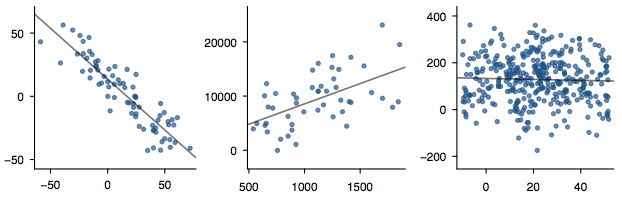
\includegraphics[scale=0.5]{ExampleSLR.png} \\[0.5cm]
  \end{center}  
{\tiny{Source: Diaz et. al. (2011, 216)}}
}

\frame{
  \frametitle{Be Careful of Non-Linear Relationships}
  \begin{center}
    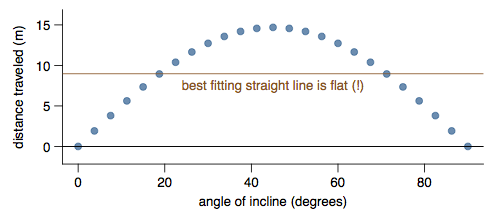
\includegraphics[scale=0.5]{NonLinear.png} \\[0.5cm]
  \end{center}  
{\tiny{Source: Diaz et. al. (2011, 216)}}
}

\frame{
  \frametitle{In fact\ldots}
  In fact, if you find a perfectly linear or almost perfectly linear relationship in social science research, you probably have a {\bf{problem}}. \\[0.5cm]
  You are probably have two variables that are measuring the same thing or almost the {\bf{same thing}}.
}

\begin{frame}[fragile]
\begin{knitrout}
\definecolor{shadecolor}{rgb}{0.969, 0.969, 0.969}\color{fgcolor}

{\centering 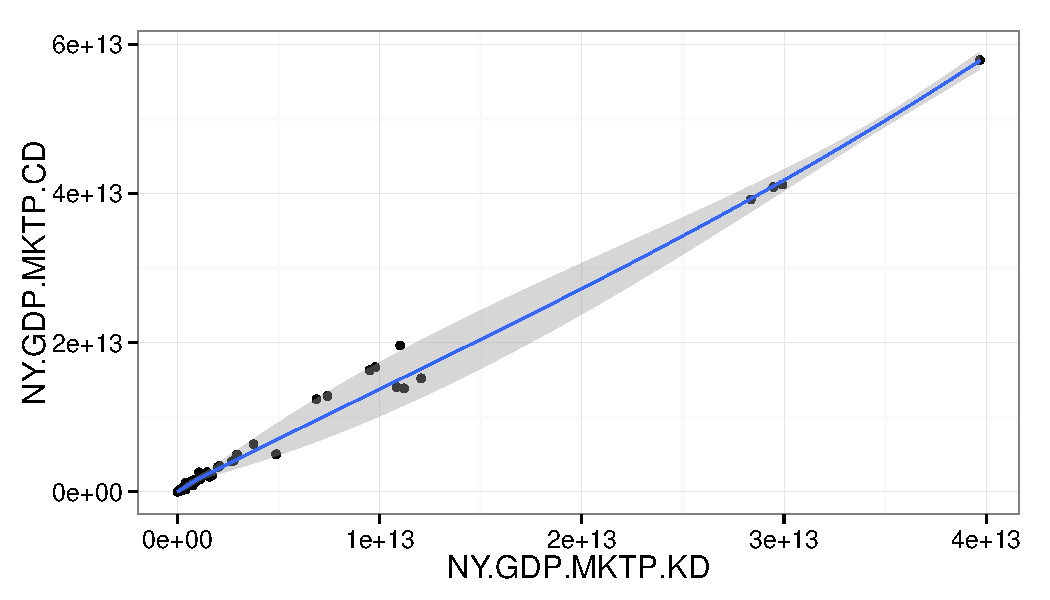
\includegraphics[width=\maxwidth]{figure/GDP1} 

}


\end{knitrout}

\end{frame}

\begin{frame}[fragile]
\begin{knitrout}
\definecolor{shadecolor}{rgb}{0.969, 0.969, 0.969}\color{fgcolor}

{\centering 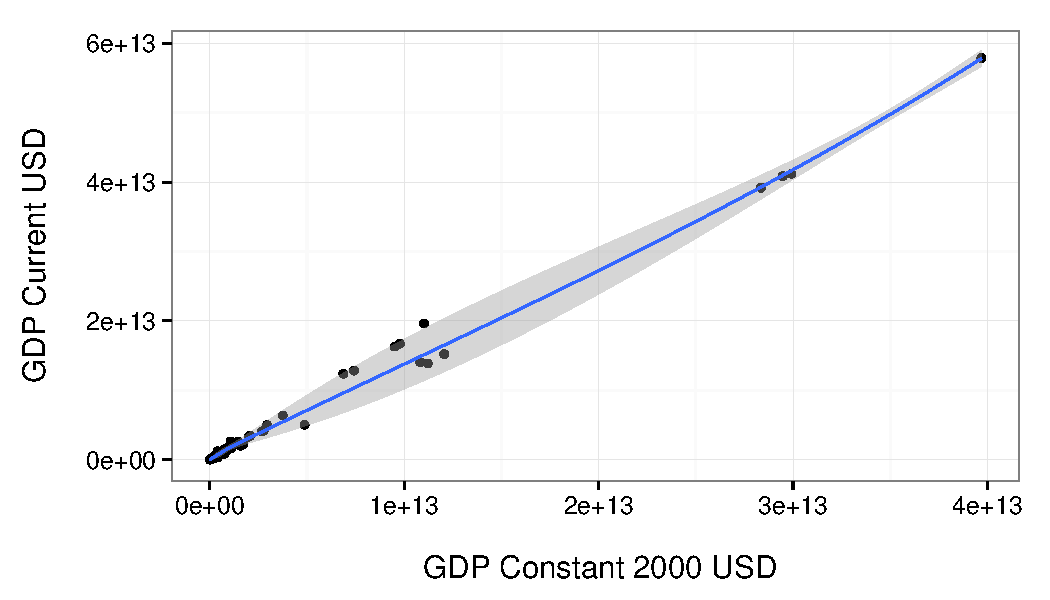
\includegraphics[width=\maxwidth]{figure/GDP2} 

}


\end{knitrout}

\end{frame}



\begin{frame}[allowframebreaks]
  \frametitle{References}
  Campbell, Frances A, Craig T Ramey, Elizabeth Pungello, Joseph Sparling, and Shari Miller-Johnson. 2002. ``Early Childhood Education: Young Adult Outcomes from the Abecedarian Project.” Applied Developmental Science 6(1): 42–57. \\[0.25cm]
  Crawley, Michael J. 2005. Statistics: An Introduction Using R. Chichester: John Wiley & Sons. Ltd. \\[0.25cm]
  Diaz, David M., Christopher D. Barr, and Mine \c{C}etinkaya-Rundel. 2011. OpenIntro Statistics. 1st ed. \url{http://www.openintro.org/stat/downloads.php}. \\[0.25cm] 
\end{frame}


\end{document}
